% !TeX encoding = UTF-8

% 载入 SJTUThesis 模版
\documentclass[degree=master, zihao=-4]{sjtuthesis}
% 选项
%   degree=[doctor|master|bachelor|course],   % 可选(默认:doctor),学位类型
%   zihao=[-4|5],                             % 可选(默认:5),正文字号大小
%   language=[chinese|english],               % 可选(默认:chinese),论文的主要语言
%   review,                                   % 可选(默认:关闭),盲审模式
%   [twoside|oneside]                         % 可选(默认:twoside),单双页模式

% 论文基本配置,加载宏包等全局配置
% !TEX root = ./main.tex

\sjtusetup{
  %
  %******************************
  % 注意:
  %   1. 配置里面不要出现空行
  %   2. 不需要的配置信息可以删除
  %******************************
  %
  % 信息录入
  %
  info = {%
    %
    % 标题
    %   可使用“\\”命令手动控制换行
    %
    title           = {DNA分子通信系统的系统模型研究},
    title*          = {A Study of Systems Modeling in DNA-Based Molecular Communications},
    %
    % 关键词
    %
    keywords        = {DNA信息分子发送器, 微观分子通信实验平台, 微观DNA分子通信建模},
    keywords*       = {DNA Information Molecule Transmitter, 
    Experimental Platform of Micro Molecular Communication, Micro DNA Molecular Communication Modeling},
    %
    % 姓名
    %
    author          = {孙文韬},
    author*         = {Wentao\quad{}Sun},
    %
    % 指导教师
    %
    supervisor      = {闫浩},
    supervisor*     = {Hao Yan},
    %
    % 副指导教师
    %
    % assisupervisor  = {某某教授},
    % assisupervisor* = {Prof. Uom Uom},
    %
    % 学号
    %
    id              = {516030910265},
    %
    % 学位
    %   本科生不需要填写
    %
    degree          = {工学学士},
    degree*         = {Bachelor of Engineering},
    %
    % 专业
    %
    major           = {测控技术与仪器},
    major*          = {Measurement and Control Technology and Instrument Science},
    %
    % 所属院系
    %
    department      = {仪器科学与工程系},
    department*     = {Depart of Instrument Science and Engineering},
    %
    % 课程名称
    %   仅课程论文适用
    %
    coursename      = {某某课程},
    %
    % 答辩日期
    %   使用 ISO 格式;默认为当前时间
    %
    % date            = {2014-12-17},
    %
    % 资助基金
    %
    % fund  = {
    %           {国家 973 项目 (No. 2025CB000000)},
    %           {国家自然科学基金 (No. 81120250000)},
    %         },
    % fund* = {
    %           {National Basic Research Program of China (Grant No. 2025CB000000)},
    %           {National Natural Science Foundation of China (Grant No. 81120250000)},
    %         },
  },
  %
  % 格式设置
  %
  format = {%
    %
    % 本科论文页眉 logo 颜色
    %   默认为黑色
    %
    % header-logo-color = red,
  },
  %
  % 名称设置
  %
  name = {%
    % publications      = {攻读学位期间完成的论文},
  },
}

% 参考文献支持宏包
\usepackage[backend=biber,style=gb7714-2015,gbpub=false,gbpunctin=false]{biblatex}
% 导入参考文献数据库
\addbibresource{bibdata/thesis.bib}

% 定义图片文件目录与扩展名
\graphicspath{{figures/}}
\DeclareGraphicsExtensions{.pdf,.eps,.png,.jpg,.jpeg}

% 确定浮动对象的位置,可以使用 [H],强制将浮动对象放到这里(可能效果很差)
\usepackage{float}

% 固定宽度的表格
\usepackage{tabularx}

% 表格中支持跨行
\usepackage{multirow}

% 表格中数字按小数点对齐
\usepackage{dcolumn}
\newcolumntype{d}[1]{D{.}{.}{#1}}

% 附带脚注的表格
\usepackage{threeparttable}

% 算法环境宏包
\usepackage[ruled,vlined,linesnumbered]{algorithm2e}
% \usepackage{algorithm}

% 代码环境宏包
\usepackage{listings}
\lstnewenvironment{codeblock}[1][]
  {\lstset{style=lstStyleCode,#1}}{}

% 国际单位制宏包
\usepackage{siunitx}

% 定理环境宏包
\usepackage{ntheorem}
% \usepackage{amsthm}

% 绘图宏包
\usepackage{tikz}

% 化学方程式宏包
\usepackage[version=4]{mhchem}

%tikz宏包
\usepackage{tikz}

% 一些文档中用到的 logo
\usepackage{hologo}
\newcommand{\XeTeX}{\hologo{XeTeX}}
\newcommand{\BibLaTeX}{\textsc{Bib}\LaTeX}

% 借用 ltxdoc 里面的几个命令。
\def\cmd#1{\cs{\expandafter\cmd@to@cs\string#1}}
\def\cmd@to@cs#1#2{\char\number`#2\relax}
\DeclareRobustCommand\cs[1]{\texttt{\char`\\#1}}

\newcommand*{\meta}[1]{{%
  \ensuremath{\langle}\rmfamily\itshape#1\/\ensuremath{\rangle}}}
\providecommand\marg[1]{%
  {\ttfamily\char`\{}\meta{#1}{\ttfamily\char`\}}}
\providecommand\oarg[1]{%
  {\ttfamily[}\meta{#1}{\ttfamily]}}
\providecommand\parg[1]{%
  {\ttfamily(}\meta{#1}{\ttfamily)}}
\providecommand\pkg[1]{{\sffamily#1}}

% 自定义命令

% E-mail
\newcommand{\email}[1]{\href{mailto:#1}{\texttt{#1}}}

% hyperref 宏包在最后调用
\usepackage{hyperref}


\begin{document}

%TC:ignore

% 无编号内容:中英文论文封面、授权页
\maketitlepage
\makeorigpage*
\makeauthpage[scans/authorization.pdf]

% 使用罗马数字对前言编号
\frontmatter

% 摘要
% !TEX root = ../main.tex

\begin{abstract}
  中文摘要应该将学位论文的内容要点简短明了地表达出来,应该包含论文中的基本信息,
  体现科研工作的核心思想。摘要内容应涉及本项科研工作的目的和意义、研究方法、研究
  成果、结论及意义。注意突出学位论文中具有创新性的成果和新见解的部分。摘要中不宜
  使用公式、化学结构式、图表和非公知公用的符号和术语,不标注引用文献编号。硕士学
  位论文中文摘要字数为 500 字左右,博士学位论文中文摘要字数为 800 字左右。英文摘
  要内容应与中文摘要内容一致。

  摘要页的下方注明本文的关键词(4~6个)。
\end{abstract}

\begin{abstract*}
  Shanghai Jiao Tong University (SJTU) is a key university in China. SJTU was
  founded in 1896. It is one of the oldest universities in China. The University
  has nurtured large numbers of outstanding figures include JIANG Zemin, DING
  Guangen, QIAN Xuesen, Wu Wenjun, WANG An, etc.

  SJTU has beautiful campuses, Bao Zhaolong Library, Various laboratories. It
  has been actively involved in international academic exchange programs. It is
  the center of CERNet in east China region, through computer networks, SJTU has
  faster and closer connection with the world.
\end{abstract*}


% 目录、插图目录、表格目录
\tableofcontents
\listoffigures*
\listoftables*
\listofalgorithms*

% 主要符号、缩略词对照表
% !TEX root = ../main.tex

\begin{nomenclature*}
\label{chap:symb}

\begin{longtable}{rl}
  $\epsilon$    & 介电常数 \\  
  $\mu$         & 磁导率 \\
\end{longtable}

\end{nomenclature*}


%TC:endignore

% 使用阿拉伯数字对正文编号
\mainmatter

% 正文内容
% !TEX root = ../main.tex

\chapter{简介}

这是 \sjtuthesis 的示例文档,基本上覆盖了模板中所有格式的设置。建议大家在使用模
板之前,除了阅读《\sjtuthesis\ 使用文档》,这个示例文档也最好能看一看。

\section{二级标题}

\subsection{三级标题}

\subsubsection{四级标题}

Lorem ipsum dolor sit amet, consectetur adipiscing elit, sed do eiusmod tempor
incididunt ut labore et dolore magna aliqua. Ut enim ad minim veniam, quis
nostrud exercitation ullamco laboris nisi ut aliquip ex ea commodo consequat.
Duis aute irure dolor in reprehenderit in voluptate velit esse cillum dolore eu
fugiat nulla pariatur. Excepteur sint occaecat cupidatat non proident, sunt in
culpa qui officia deserunt mollit anim id est laborum.

\section{脚注}

Lorem ipsum dolor sit amet, consectetur adipiscing elit, sed do eiusmod tempor
incididunt ut labore et dolore magna aliqua. \footnote{Ut enim ad minim veniam,
quis nostrud exercitation ullamco laboris nisi ut aliquip ex ea commodo
consequat. Duis aute irure dolor in reprehenderit in voluptate velit esse cillum
dolore eu fugiat nulla pariatur.}

\section{字体}


上海交通大学是我国历史最悠久的高等学府之一,是教育部直属、教育部与上海市共建的全
国重点大学,是国家“七五”、“八五”重点建设和“211 工程”、“985 工程”的首批建
设高校。经过 115 年的不懈努力,上海交通大学已经成为一所“综合性、研究型、国际化”
的国内一流、国际知名大学,并正在向世界一流大学稳步迈进。 

{\songti 十九世纪末,甲午战败,民族危难。中国近代著名实业家、教育家盛宣怀和一批
  有识之士秉持“自强首在储才,储才必先兴学”的信念,于 1896 年在上海创办了交通大
  学的前身——南洋公学。建校伊始,学校即坚持“求实学,务实业”的宗旨,以培养“第
  一等人才”为教育目标,精勤进取,笃行不倦,在二十世纪二三十年代已成为国内著名的
  高等学府,被誉为“东方MIT”。抗战时期,广大师生历尽艰难,移转租界,内迁重庆,
  坚持办学,不少学生投笔从戎,浴血沙场。解放前夕,广大师生积极投身民主革命,学校
  被誉为“民主堡垒”。}

{\heiti 新中国成立初期,为配合国家经济建设的需要,学校调整出相当一部分优势专业、
  师资设备,支持国内兄弟院校的发展。五十年代中期,学校又响应国家建设大西北的号
  召,根据国务院决定,部分迁往西安,分为交通大学上海部分和西安部分。1959 年 3月
  两部分同时被列为全国重点大学,7 月经国务院批准分别独立建制,交通大学上海部分启
  用“上海交通大学”校名。历经西迁、两地办学、独立办学等变迁,为构建新中国的高等
  教育体系,促进社会主义建设做出了重要贡献。六七十年代,学校先后归属国防科工委和
  六机部领导,积极投身国防人才培养和国防科研,为“两弹一星”和国防现代化做出了
  巨大贡献。}

{\kaishu 改革开放以来,学校以“敢为天下先”的精神,大胆推进改革:率先组成教授代
  表团访问美国,率先实行校内管理体制改革,率先接受海外友人巨资捐赠等,有力地推动
  了学校的教学科研改革。1984 年,邓小平同志亲切接见了学校领导和师生代表,对学校
  的各项改革给予了充分肯定。在国家和上海市的大力支持下,学校以“上水平、创一流”
  为目标,以学科建设为龙头,先后恢复和兴建了理科、管理学科、生命学科、法学和人文
  学科等。1999 年,上海农学院并入;2005 年,与上海第二医科大学强强合并。至此,学
  校完成了综合性大学的学科布局。近年来,通过国家“985 工程”和“211 工程”的建
  设,学校高层次人才日渐汇聚,科研实力快速提升,实现了向研究型大学的转变。与此同
  时,学校通过与美国密西根大学等世界一流大学的合作办学,实施国际化战略取得重要突
  破。1985 年开始闵行校区建设,历经 20 多年,已基本建设成设施完善,环境优美的现
  代化大学校园,并已完成了办学重心向闵行校区的转移。学校现有徐汇、闵行、法华、七
  宝和重庆南路(卢湾)5 个校区,总占地面积 4840 亩。通过一系列的改革和建设,学校
  的各项办学指标大幅度上升,实现了跨越式发展,整体实力显著增强,为建设世界一流大
  学奠定了坚实的基础。}

{\fangsong 交通大学始终把人才培养作为办学的根本任务。一百多年来,学校为国家和社
  会培养了 20余万各类优秀人才,包括一批杰出的政治家、科学家、社会活动家、实业
  家、工程技术专家和医学专家,如江泽民、陆定一、丁关根、汪道涵、钱学森、吴文俊、
  徐光宪、张光斗、黄炎培、邵力子、李叔同、蔡锷、邹韬奋、陈敏章、王振义、陈竺等。
  在中国科学院、中国工程院院士中,有 200 余位交大校友;在国家 23 位“两弹一星”
  功臣中,有 6 位交大校友;在 18 位国家最高科学技术奖获得者中,有 3 位来自交大。
  交大创造了中国近现代发展史上的诸多“第一”:中国最早的内燃机、最早的电机、最早
  的中文打字机等;新中国第一艘万吨轮、第一艘核潜艇、第一艘气垫船、第一艘水翼艇、
  自主设计的第一代战斗机、第一枚运载火箭、第一颗人造卫星、第一例心脏二尖瓣分离
  术、第一例成功移植同种原位肝手术、第一例成功抢救大面积烧伤病人手术等,都凝聚着
  交大师生和校友的心血智慧。改革开放以来,一批年轻的校友已在世界各地、各行各业崭
  露头角。}

{\ifcsname lishu\endcsname\lishu\else[无 \cs{lishu} 字体。]\fi 截至 2011 年 12
  月 31 日,学校共有 24 个学院 / 直属系(另有继续教育学院、技术学院和国际教育学
  院),19 个直属单位,12 家附属医院,全日制本科生 16802 人、研究生24495 人(其
  中博士研究生 5059 人);有专任教师 2979 名,其中教授 835 名;中国科学院院士 15
  名,中国工程院院士 20 名,中组部“千人计划”49 名,“长江学者”95 名,国家杰出
  青年基金获得者 80 名,国家重点基础研究发展计划(973 计划)首席科学家 24名,国
  家重大科学研究计划首席科学家 9名,国家基金委创新研究群体 6 个,教育部创新团队
  17 个。}

{\ifcsname youyuan\endcsname\youyuan\else[无 \cs{youyuan} 字体。]\fi 学校现有本
  科专业 68 个,涵盖经济学、法学、文学、理学、工学、农学、医学、管理学和艺术等九
  个学科门类;拥有国家级教学及人才培养基地 7 个,国家级校外实践教育基地 5个,国
  家级实验教学示范中心 5 个,上海市实验教学示范中心 4 个;有国家级教学团队 8个,
  上海市教学团队 15 个;有国家级教学名师 7 人,上海市教学名师 35 人;有国家级精
  品课程 46 门,上海市精品课程 117 门;有国家级双语示范课程 7 门;2001、2005 和
  2009 年,作为第一完成单位,共获得国家级教学成果 37 项、上海市教学成果 157
  项。}

% !TeX root = ../main.tex

\chapter{浮动体}

\section{插图}

插图功能是利用 \TeX\ 的特定编译程序提供的机制实现的,不同的编译程序支持不同的图
形方式。有的同学可能听说“\LaTeX\ 只支持 EPS”,事实上这种说法是不准确的。\XeTeX
可以很方便地插入 EPS、PDF、PNG、JPEG 格式的图片。

一般图形都是处在浮动环境中。之所以称为浮动是指最终排版效果图形的位置不一定与源文
件中的位置对应,这也是刚使用 \LaTeX\ 同学可能遇到的问题。如果要强制固定浮动图形
的位置,请使用 \pkg{float} 宏包,它提供了 \texttt{[H]} 参数。

\subsection{单个图形}

图要有图题,研究生图题采用中英文对照,并置于图的编号之后,图的编号和图题应置于图
下方的居中位置。引用图应在图题右上角标出文献来源。当插图中组成部件由数字或字母等
编号表示时,可在插图下方添加图注进行说明,如图~\ref{fig:cn_100t} 所示。

\begin{figure}[!htp]
  \centering
  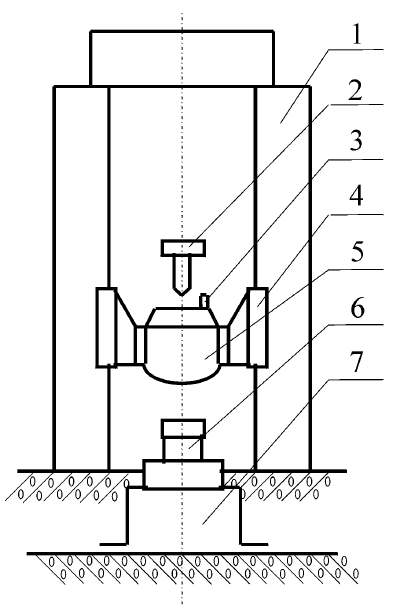
\includegraphics[width=4cm]{cn_100t.png} \\
    1.立柱 2.提升释放机构 3.标准冲击加速度计 \\
    4.导轨 5.重锤 6.被校力传感器 7.底座 \\
  \bicaption[出现在插图索引中]
    {单个图形示例\cite{he1999}。如果表格的标题很长,那么在表格索引中就会很不美观。可
      以在前面用中括号写一个简短的标题,这个标题会出现在索引中。}
    {Stay hungry, stay foolish.}
 \label{fig:cn_100t}
\end{figure}

Lorem ipsum dolor sit amet, consectetur adipisici elit, sed do eiusmod tempor
incididunt ut labore et dolore magna aliqua. Ut enim ad minim veniam, quis
nostrud exercitation ullamco laboris nisi ut aliquip ex ea commodo consequat.
Duis aute irure dolor in reprehenderit in voluptate velit esse cillum dolore eu
fugiat nulla pariatur. Excepteur sint occaecat cupidatat non proident, sunt in
culpa qui officia deserunt mollit anim id est laborum.

\subsection{多个图形}

简单插入多个图形的例子如图~\ref{fig:SRR} 所示。这两个水平并列放置的子图共用一个
图形计数器,没有各自的子图题。

\begin{figure}[!htp]
  \centering
  
\includegraphics[height=2cm]{sjtu-vi-badge-blue.pdf}
  \hspace{1cm}
  
\includegraphics[height=2cm]{sjtu-vi-badge-blue.pdf}
  \bicaption{中文题图}{English caption}
  \label{fig:SRR}
\end{figure}

如果多个图形相互独立,并不共用一个图形计数器,那么用 \texttt{minipage} 或者
\texttt{parbox} 就可以,如图~\ref{fig:parallel1} 与图~\ref{fig:parallel2}。

\begin{figure}[!htp]
\begin{minipage}{0.48\textwidth}
  \centering
  
\includegraphics[height=1.5cm]{sjtu-vi-name-blue.pdf}
  \caption{并排第一个图}
  \label{fig:parallel1}
\end{minipage}\hfill
\begin{minipage}{0.48\textwidth}
  \centering
  
\includegraphics[height=1.5cm]{sjtu-vi-name-blue.pdf}
  \caption{并排第二个图}
  \label{fig:parallel2}
\end{minipage}
\end{figure}

Lorem ipsum dolor sit amet, consectetur adipisici elit, sed do eiusmod tempor
incididunt ut labore et dolore magna aliqua. Ut enim ad minim veniam, quis
nostrud exercitation ullamco laboris nisi ut aliquip ex ea commodo consequat.
Duis aute irure dolor in reprehenderit in voluptate velit esse cillum dolore eu
fugiat nulla pariatur. Excepteur sint occaecat cupidatat non proident, sunt in
culpa qui officia deserunt mollit anim id est laborum.

如果要为共用一个计数器的多个子图添加子图题,建议使用较新的 \pkg{subcaption}宏
包,不建议使用 \pkg{subfigure} 或 \pkg{subfig} 等宏包。

推荐使用 \pkg{subcaption} 宏包的 \cs{subcaptionbox} 并排子图,子图题置于子图之
下,子图号用 a)、b) 等表示。也可以使用 \pkg{subcaption} 宏包的 \cs{subcaption}
(放在 minipage中,用法同 \cs{caption})。

搭配 \pkg{bicaption} 宏包时,可以启用 \cs{subcaptionbox} 和 \cs{subcaption} 的双
语变种 \cs{bisubcaptionbox} 和 \cs{bisubcaption},如图~\ref{fig:bisubcaptionbox}
所示。

\begin{figure}[!hbtp]
  \centering
  \bisubcaptionbox{$R_3 = 1.5\text{mm}$ 时轴承的压力分布云图}%
                  {Pressure contour of bearing when $R_3 = 1.5\text{mm}$}%
                  [6.4cm]{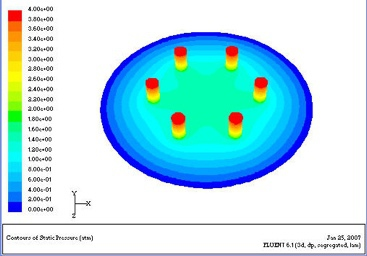
\includegraphics[height=2.5cm]{pressure15.jpg}}
  \hspace{1cm}
  \bisubcaptionbox{$R_3 = 2.5\text{mm}$ 时轴承的压力分布云图}%
                  {Pressure contour of bearing when $R_3 = 2.5\text{mm}$}%
                  [6.4cm]{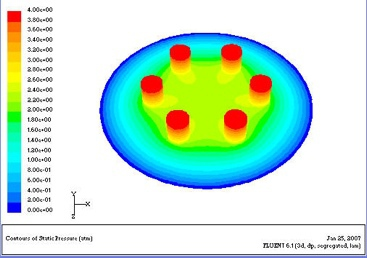
\includegraphics[height=2.5cm]{/pressure25.jpg}}
  \bicaption{包含子图题的范例(使用 subcaptionbox)}
            {Example with subcaptionbox}
  \label{fig:bisubcaptionbox}
\end{figure}

\pkg{subcaption} 宏包也提供了 \pkg{subfigure} 和 \pkg{subtable} 环境,如
图~\ref{fig:subfigure}。

\begin{figure}[!htp]
  \centering
  \begin{subfigure}{0.3\textwidth}
    \centering
    
\includegraphics[height=2cm]{sjtu-vi-badge-blue.pdf}
    \caption{校徽}
  \end{subfigure}
  \hspace{1cm}
  \begin{subfigure}{0.4\textwidth}
    \centering
    
\includegraphics[height=1.5cm]{sjtu-vi-name-blue.pdf}
    \caption{校名。注意这个图略矮些,subfigure 中同一行的子图在顶端对齐。}
  \end{subfigure}
  \caption{包含子图题的范例(使用 subfigure)}
  \label{fig:subfigure}
\end{figure}

Lorem ipsum dolor sit amet, consectetur adipisici elit, sed do eiusmod tempor
incididunt ut labore et dolore magna aliqua. Ut enim ad minim veniam, quis
nostrud exercitation ullamco laboris nisi ut aliquip ex ea commodo consequat.
Duis aute irure dolor in reprehenderit in voluptate velit esse cillum dolore eu
fugiat nulla pariatur. Excepteur sint occaecat cupidatat non proident, sunt in
culpa qui officia deserunt mollit anim id est laborum.

\section{表格}

\subsection{基本表格}

编排表格应简单明了,表达一致,明晰易懂,表文呼应、内容一致。表题置于表上,研究生
学位论文可以用中、英文两种文字居中排写,中文在上,也可以只用中文。

表格的编排建议采用国际通行的三线表\footnote{三线表,以其形式简洁、功能分明、阅读
方便而在科技论文中被推荐使用。三线表通常只有 3 条线,即顶线、底线和栏目线,没有
竖线。}。三线表可以使用 \pkg{booktabs} 提供的 \cs{toprule}、\cs{midrule} 和
\cs{bottomrule}。它们与 \pkg{longtable} 能很好的配合使用。

\begin{table}[!hpt]
  \caption[一个颇为标准的三线表]{一个颇为标准的三线表\footnotemark}
  \label{tab:firstone}
  \centering
  \begin{tabular}{@{}llr@{}} \toprule
    \multicolumn{2}{c}{Item} \\ \cmidrule(r){1-2}
    Animal & Description & Price (\$)\\ \midrule
    Gnat  & per gram  & 13.65 \\
          & each      & 0.01 \\
    Gnu   & stuffed   & 92.50 \\
    Emu   & stuffed   & 33.33 \\
    Armadillo & frozen & 8.99 \\ \bottomrule
  \end{tabular}
\end{table}
\footnotetext{这个例子来自
  \href{https://mirrors.sjtug.sjtu.edu.cn/ctan/macros/latex/contrib/booktabs/booktabs.pdf}%
  {《Publication quality tables in LaTeX》}(\pkg{booktabs} 宏包的文档)。这也是
  一个在表格中使用脚注的例子,请留意与 \pkg{threeparttable} 实现的效果有何不
  同。}

\subsection{复杂表格}

我们经常会在表格下方标注数据来源,或者对表格里面的条目进行解释。可以用
\pkg{threeparttable} 实现带有脚注的表格,如表~\ref{tab:footnote}。

\begin{table}[!htpb]
  \bicaption{一个带有脚注的表格的例子}{A Table with footnotes}
  \label{tab:footnote}
  \centering
  \begin{threeparttable}[b]
     \begin{tabular}{ccd{4}cccc}
      \toprule
      \multirow{2}*{total} & \multicolumn{2}{c}{20\tnote{a}} & \multicolumn{2}{c}{40} & \multicolumn{2}{c}{60} \\
      \cmidrule(lr){2-3}\cmidrule(lr){4-5}\cmidrule(lr){6-7}
      & www & \multicolumn{1}{c}{k} & www & k & www & k \\ % 使用说明符 d 的列会自动进入数学模式,使用 \multicolumn 对文字表头做特殊处理
      \midrule
      & $\underset{(2.12)}{4.22}$ & 120.0140\tnote{b} & 333.15 & 0.0411 & 444.99 & 0.1387 \\
      & 168.6123 & 10.86 & 255.37 & 0.0353 & 376.14 & 0.1058 \\
      & 6.761    & 0.007 & 235.37 & 0.0267 & 348.66 & 0.1010 \\
      \bottomrule
    \end{tabular}
    \begin{tablenotes}
    \item [a] the first note.% or \item [a]
    \item [b] the second note.% or \item [b]
    \end{tablenotes}
  \end{threeparttable}
\end{table}

Lorem ipsum dolor sit amet, consectetur adipisici elit, sed do eiusmod tempor
incididunt ut labore et dolore magna aliqua. Ut enim ad minim veniam, quis
nostrud exercitation ullamco laboris nisi ut aliquip ex ea commodo consequat.
Duis aute irure dolor in reprehenderit in voluptate velit esse cillum dolore eu
fugiat nulla pariatur. Excepteur sint occaecat cupidatat non proident, sunt in
culpa qui officia deserunt mollit anim id est laborum.

如某个表需要转页接排,可以用 \pkg{longtable} 实现。接排时表题省略,表头应重复书
写,并在右上方写“续表 xx”,如表~\ref{tab:performance}。

\begin{longtable}[c]{c*{6}{r}}
  \bicaption{实验数据}{Experimental data}
  \label{tab:performance} \\
  \toprule
  测试程序 & \multicolumn{1}{c}{正常运行} & \multicolumn{1}{c}{同步}
    & \multicolumn{1}{c}{检查点} & \multicolumn{1}{c}{卷回恢复}
    & \multicolumn{1}{c}{进程迁移} & \multicolumn{1}{c}{检查点} \\
   & \multicolumn{1}{c}{时间 (s)} & \multicolumn{1}{c}{时间 (s)}
    & \multicolumn{1}{c}{时间 (s)} & \multicolumn{1}{c}{时间 (s)}
    & \multicolumn{1}{c}{时间 (s)} &  文件(KB)\\
  \midrule
  \endfirsthead
  \multicolumn{7}{r}{续表~\thetable} \\
  \toprule
  测试程序 & \multicolumn{1}{c}{正常运行} & \multicolumn{1}{c}{同步}
    & \multicolumn{1}{c}{检查点} & \multicolumn{1}{c}{卷回恢复}
    & \multicolumn{1}{c}{进程迁移} & \multicolumn{1}{c}{检查点} \\
   & \multicolumn{1}{c}{时间 (s)} & \multicolumn{1}{c}{时间 (s)}
    & \multicolumn{1}{c}{时间 (s)} & \multicolumn{1}{c}{时间 (s)}
    & \multicolumn{1}{c}{时间 (s)}&  文件(KB)\\
  \midrule
  \endhead
  \hline
  \multicolumn{7}{r}{续下页}
  \endfoot
  \endlastfoot
  CG.A.2 & 23.05 & 0.002 & 0.116 & 0.035 & 0.589 & 32491 \\
  CG.A.4 & 15.06 & 0.003 & 0.067 & 0.021 & 0.351 & 18211 \\
  CG.A.8 & 13.38 & 0.004 & 0.072 & 0.023 & 0.210 & 9890 \\
  CG.B.2 & 867.45 & 0.002 & 0.864 & 0.232 & 3.256 & 228562 \\
  CG.B.4 & 501.61 & 0.003 & 0.438 & 0.136 & 2.075 & 123862 \\
  CG.B.8 & 384.65 & 0.004 & 0.457 & 0.108 & 1.235 & 63777 \\
  MG.A.2 & 112.27 & 0.002 & 0.846 & 0.237 & 3.930 & 236473 \\
  MG.A.4 & 59.84 & 0.003 & 0.442 & 0.128 & 2.070 & 123875 \\
  MG.A.8 & 31.38 & 0.003 & 0.476 & 0.114 & 1.041 & 60627 \\
  MG.B.2 & 526.28 & 0.002 & 0.821 & 0.238 & 4.176 & 236635 \\
  MG.B.4 & 280.11 & 0.003 & 0.432 & 0.130 & 1.706 & 123793 \\
  MG.B.8 & 148.29 & 0.003 & 0.442 & 0.116 & 0.893 & 60600 \\
  LU.A.2 & 2116.54 & 0.002 & 0.110 & 0.030 & 0.532 & 28754 \\
  LU.A.4 & 1102.50 & 0.002 & 0.069 & 0.017 & 0.255 & 14915 \\
  LU.A.8 & 574.47 & 0.003 & 0.067 & 0.016 & 0.192 & 8655 \\
  LU.B.2 & 9712.87 & 0.002 & 0.357 & 0.104 & 1.734 & 101975 \\
  LU.B.4 & 4757.80 & 0.003 & 0.190 & 0.056 & 0.808 & 53522 \\
  LU.B.8 & 2444.05 & 0.004 & 0.222 & 0.057 & 0.548 & 30134 \\
  EP.A.2 & 123.81 & 0.002 & 0.010 & 0.003 & 0.074 & 1834 \\
  EP.A.4 & 61.92 & 0.003 & 0.011 & 0.004 & 0.073 & 1743 \\
  EP.A.8 & 31.06 & 0.004 & 0.017 & 0.005 & 0.073 & 1661 \\
  EP.B.2 & 495.49 & 0.001 & 0.009 & 0.003 & 0.196 & 2011 \\
  EP.B.4 & 247.69 & 0.002 & 0.012 & 0.004 & 0.122 & 1663 \\
  EP.B.8 & 126.74 & 0.003 & 0.017 & 0.005 & 0.083 & 1656 \\
  SP.A.2 & 123.81 & 0.002 & 0.010 & 0.003 & 0.074 & 1854 \\
  SP.A.4 & 51.92 & 0.003 & 0.011 & 0.004 & 0.073 & 1543 \\
  SP.A.8 & 31.06 & 0.004 & 0.017 & 0.005 & 0.073 & 1671 \\
  SP.B.2 & 495.49 & 0.001 & 0.009 & 0.003 & 0.196 & 2411 \\
  SP.B.4 & 247.69 & 0.002 & 0.014 & 0.006 & 0.152 & 2653 \\
  SP.B.8 & 126.74 & 0.003 & 0.017 & 0.005 & 0.082 & 1755 \\
  \bottomrule
\end{longtable}

\section{算法环境}

算法环境可以使用 \pkg{algorithms} 宏包或者较新的 \pkg{algorithm2e} 实现。
算法~\ref{algo:algorithm} 是一个使用 \pkg{algorithm2e} 的例子。关于排版算法环境
的具体方法,请阅读相关宏包的官方文档。

\begin{algorithm}[htb]
  \caption{算法示例}
  \label{algo:algorithm}
  \small
  \SetAlgoLined
  \KwData{this text}
  \KwResult{how to write algorithm with \LaTeXe }

  initialization\;
  \While{not at end of this document}{
    read current\;
    \eIf{understand}{
      go to next section\;
      current section becomes this one\;
    }{
      go back to the beginning of current section\;
    }
  }
\end{algorithm}

\section{代码环境}

我们可以在论文中插入算法,但是不建议插入大段的代码。如果确实需要插入代码,建议使
用 \pkg{listings} 宏包。

\begin{codeblock}[language=C]
#include <stdio.h>
#include <unistd.h>
#include <sys/types.h>
#include <sys/wait.h>

int main() {
  pid_t pid;

  switch ((pid = fork())) {
  case -1:
    printf("fork failed\n");
    break;
  case 0:
    /* child calls exec */
    execl("/bin/ls", "ls", "-l", (char*)0);
    printf("execl failed\n");
    break;
  default:
    /* parent uses wait to suspend execution until child finishes */
    wait((int*)0);
    printf("is completed\n");
    break;
  }

  return 0;
}
\end{codeblock}

% !TEX root = ../main.tex

\chapter{数学与引用文献的标注}

\section{数学}

\subsection{数字和单位}

宏包 \pkg{siunitx} 提供了更好的数字和单位支持:
\begin{itemize}
  \item \num{12345.67890}
  \item \num{1+-2i}
  \item \num{.3e45}
  \item \num{1.654 x 2.34 x 3.430}
  \item \si{kg.m.s^{-1}}
  \item \si{\micro\meter} $\si{\micro\meter}$
  \item \si{\ohm} $\si{\ohm}$
  \item \numlist{10;20}
  \item \numlist{10;20;30}
  \item \SIlist{0.13;0.67;0.80}{\milli\metre}
  \item \numrange{10}{20}
  \item \SIrange{10}{20}{\degreeCelsius}
\end{itemize}

\subsection{数学符号和公式}

微分符号 $\dif$ 应使用正体,本模板提供了 \cs{dif} 命令。除此之外,模板还提供了一
些命令方便使用:
\begin{itemize}
  \item 圆周率 $\uppi$:\verb|\uppi|
  \item 自然对数的底 $\upe$:\verb|\upe|
  \item 虚数单位 $\upi$, $\upj$:\verb|\upi| \verb|\upj|
\end{itemize}

公式应另起一行居中排版。公式后应注明编号,按章顺序编排,编号右端对齐。
\begin{equation}
  \upe^{\upi\uppi} + 1 = 0,
\end{equation}
\begin{equation}
  \frac{\dif^2 u}{\dif t^2} = \int f(x) \dif x.
\end{equation}

公式末尾是需要添加标点符号的,至于用逗号还是句号,取决于公式下面一句是接着公式说的,还是另起一句。
\begin{equation}
		\frac{2h}{\pi}\int_{0}^{\infty}\frac{\sin\left( \omega\delta \right)}{\omega}
		\cos\left( \omega x \right) \dif\omega = 
		\begin{cases}
				h, \ \left| x \right| < \delta, \\
				\frac{h}{2}, \ x = \pm \delta, \\
				0, \ \left| x \right| > \delta.
		\end{cases}
\end{equation}
公式较长时最好在等号“$=$”处转行。
\begin{align}
    & I (X_3; X_4) - I (X_3; X_4 \mid X_1) - I (X_3; X_4 \mid X_2) \nonumber \\
  = & [I (X_3; X_4) - I (X_3; X_4 \mid X_1)] - I (X_3; X_4 \mid \tilde{X}_2) \\
  = & I (X_1; X_3; X_4) - I (X_3; X_4 \mid \tilde{X}_2).
\end{align}

如果在等号处转行难以实现,也可在 $+$、$-$、$\times$、$\div$运算符号处转行,转行
时运算符号仅书写于转行式前,不重复书写。
\begin{multline}
  \frac{1}{2} \Delta (f_{ij} f^{ij}) =
    2 \left(\sum_{i<j} \chi_{ij}(\sigma_{i} - \sigma_{j})^{2}
    + f^{ij} \nabla_{j} \nabla_{i} (\Delta f) \right. \\
  \left. + \nabla_{k} f_{ij} \nabla^{k} f^{ij} +
    f^{ij} f^{k} \left[2\nabla_{i}R_{jk}
    - \nabla_{k} R_{ij} \right] \vphantom{\sum_{i<j}} \right).
\end{multline}

\subsection{定理环境}

示例文件中使用 \pkg{ntheorem} 宏包配置了定理、引理和证明等环境。用户也可以使用
\pkg{amsthm} 宏包。

这里举一个“定理”和“证明”的例子。
\begin{theorem}[留数定理]
\label{thm:res}
  假设 $U$ 是复平面上的一个单连通开子集,$a_1, \ldots, a_n$ 是复平面上有限个点,
  $f$ 是定义在 $U \backslash \{a_1, \ldots, a_n\}$ 上的全纯函数,如果 $\gamma$
  是一条把 $a_1, \ldots, a_n$ 包围起来的可求长曲线,但不经过任何一个 $a_k$,并且
  其起点与终点重合,那么:

  \begin{equation}
    \label{eq:res}
    \ointop_\gamma f(z)\, \dif z = 2\uppi \upi \sum_{k=1}^n \operatorname{I}(\gamma, a_k) \operatorname{Res}(f, a_k).
  \end{equation}

  如果 $\gamma$ 是若尔当曲线,那么 $\operatorname{I}(\gamma, a_k) = 1$,因此:

  \begin{equation}
    \label{eq:resthm}
    \ointop_\gamma f(z)\, \dif z = 2\uppi \upi \sum_{k=1}^n \operatorname{Res}(f, a_k).
  \end{equation}

  在这里,$\operatorname{Res}(f, a_k)$ 表示 $f$ 在点 $a_k$ 的留数,
  $\operatorname{I}(\gamma, a_k)$ 表示 $\gamma$ 关于点 $a_k$ 的卷绕数。卷绕数是
  一个整数,它描述了曲线 $\gamma$ 绕过点 $a_k$ 的次数。如果 $\gamma$ 依逆时针方
  向绕着 $a_k$ 移动,卷绕数就是一个正数,如果 $\gamma$ 根本不绕过 $a_k$,卷绕数
  就是零。

  定理~\ref{thm:res} 的证明。

  \begin{proof}
    首先,由……

    其次,……

    所以……
  \end{proof}
\end{theorem}

\section{引用文献的标注}

按照教务处的要求,参考文献外观应符合国标 GB/T 7714 的要求。模版使用 \BibLaTeX\
配合 \pkg{biblatex-gb7714-2015} 样式包
\footnote{\url{https://www.ctan.org/pkg/biblatex-gb7714-2015}}
控制参考文献的输出样式,后端采用 \pkg{biber} 管理文献。

请注意 \pkg{biblatex-gb7714-2015} 宏包 2016 年 9 月才加入 CTAN,如果你使用的
\TeX\ 系统版本较旧,可能没有包含 \pkg{biblatex-gb7714-2015} 宏包,需要手动安装。
\BibLaTeX\ 与 \pkg{biblatex-gb7714-2015} 目前在活跃地更新,为避免一些兼容性问
题,推荐使用较新的版本。

正文中引用参考文献时,使用 \verb|\cite{key1,key2,key3...}| 可以产生“上标引用的
参考文献”,如 \cite{Meta_CN,chen2007act,DPMG}。使用
\verb|\parencite{key1,key2,key3...}| 则可以产生水平引用的参考文献,例如
\parencite{JohnD,zhubajie,IEEE-1363}。请看下面的例子,将会穿插使用水平的和上标的
参考文献:关于书的\parencite{Meta_CN,JohnD,IEEE-1363},关于期刊的
\cite{chen2007act,chen2007ewi},会议论文 \parencite{DPMG,kocher99,cnproceed},硕
士学位论文\parencite{zhubajie,metamori2004},博士学位论文
\cite{shaheshang,FistSystem01,bai2008},标准文件 \parencite{IEEE-1363},技术报告
\cite{NPB2},电子文献 \parencite{xiaoyu2001, CHRISTINE1998},用户手册
\parencite{RManual}。

当需要将参考文献条目加入到文献表中但又不在正文中引用,可以使用
\verb|\nocite{key1,key2,key3...}|。使用 \verb|\nocite{*}| 可以将参考文献数据库中
的所有条目加入到文献表中。

% !TEX root = ../main.tex

\begin{summary}
针对分子通信领域缺少微观实验平台的瓶颈问题,
本课题组提出了以DNA为信息分子的微观分子通信实验平台
 ,并初步完成了其中关键部件的DNA信息分子的发送器与接收器的设计与实现
。然而,针对DNA分子通信,领域内并没有相关的理论研究。但是,
对实验平台的深入理解,离不开理论研究的指导。针对这个问题,
本毕业设计立足于课题组的现有的DNA分子通信实验平台,对其中DNA信息分子发送器部分开展理论研究。\\

首先,我们融合化学、物理学科的知识,利用COMSOL Multiphysics与MATLAB软件,基于电化学反应原理、化学动力学原理、粒子自由扩散与带电粒子在电场辅助下自由扩散的原理,获得了DNA信息分子发送器的三维理论模型。其次,我们利用获得的DNA信息分子发送器模型,研究了关键参数对DNA发送过程的影响,包括:激励信号与接收机位置等,并分析了关键系统参数对信息传播速度、抗干扰能力、总发送量这三个性能的影响。通过本工作的研究,课题组深入理解了DNA信息分子发送器的特征,指明了优化DNA信息分子发送器的具体方向。对进一步推进本课题组的微观分子通信实验平台的研究具有重要意义。\\

本工作的主要研究结果包含如下几个方面:

1)通过学习,了解了分子通信领域的发展现状与分子通信的基本原理。 

2)通过调研与阅读多学科文献,学习、归纳并总结了DNA信息分子发送器中关键的多层DNA结构的组装过程
、理化性质以及DNA分子的扩散运动运动过程。通过自己的理解与调研
,详细分析与讨论了DNA信息分子分解与释放过程中的电化学反应、水解反应、
电迁移及扩散过程,并最终提出DNA/$\ce{Zr^4+}$多层结构的分解与释放的原理。并
将上述多个过程表达为对应的理论方程。

3)利用两个软件,COMSOL Multiphysics 与 MATLAB,对上述DNA信息分子发送过
程进行数值仿真,仿真结果与课题组的实验数据符合度好,证明了所提出的模型的准确性与有效性。
也验证了利用COMSOL Multiphysics 与 MATLAB对电极反应、水解反应、
电泳等多个过程共同作用的仿真可以用于对DNA分子通信系统的建模。

4)对DNA信息分子发送器的系统特征进行研究,深入理解了DNA信息分子发送器的
特征,指明了优化DNA信息分子发送器的具体方向。关键结论包括:

$\bullet$讨论了激励电压信号的强度与持续时间对DNA信息分子发送过程的影响。不考虑电解热效应的情况下,
激励电压越高,系统抗码间串扰的能力越强。激励时长越短,系统抗码间串扰的能力越强。激励信号需要具备持续时间较短
、激励电压较高的特性,高电压的脉冲函数是一个理想的信号源。

$\bullet$讨论了接收机位置对系统性能的影响,获得信道中不同位置初的DNA浓度变化曲线并研究了DNA信息分子发送器
的阈值。接收机距离阴极越近,DNA浓度达到峰值的时间越短,峰值强度越大。接收机距离越短,信号传输效果越好。
短时长的信号的激励下,相同位置处,DNA浓度峰值会更早到达,峰值相对于整条曲线也会更突出。
在距离阴极 0.5$mm$的地方,我们可以达到54.5$bit/min$的最大通信速率;
在距离阴极 4.5$mm$处,我们可以达到16.7$bit/min$的最大通信频率,而在距离阴极9.5$mm$处,最大通信频率只有3.2$bit/min$。
数据说明了,基于自由扩散的通信系统,
不适合远距离通信。接收机放置在距发送机5$mm$以内这一范围内时,能达到一个较快的传输速度,
而且抗干扰能力强。在超过7$mm$这一范围后,
信号间隔必须增加到数十秒,以抑制码间串扰,而且其抗码间串扰的能力能力也会下降。

$\bullet$综合考虑平衡常数,在$\ce{OH-}$存在时,$\ce{Zr^4+}$水解反应都会发生,
由于反应速度与$c_{\ce{OH-}}$的4次方成正比,所以低$\ce{OH-}$浓度时,
反应速度极慢,在所观测的时间尺度下,可以认为不施加激励电压时反应不发生。
电化学反应的电压阈值应为2.17$V$。但实际条件下,由于电极阻抗、溶液电导率等因素的影响,
可能需要更大的电压来启动此反应。通过对激励电压与时长的控制,一个DNA/$\ce{Zr^4+}$单层可以被多次释放,
在激励电压为5$V$,激励时长为1$s$的信号作用下,每一层DNA/$\ce{Zr^4+}$单层最多可以释放6次。


\end{summary}


%TC:ignore

% 使用英文字母对附录编号
\appendix

% 附录内容,本科学位论文可以用翻译的文献替代。
% !TEX root = ../main.tex

\chapter{Maxwell Equations}

选择二维情况,有如下的偏振矢量:
\begin{subequations}
  \begin{align}
    {\bf E} &= E_z(r, \theta) \hat{\bf z}, \\
    {\bf H} &= H_r(r, \theta) \hat{\bf r} + H_\theta(r, \theta) \hat{\bm\theta}.
  \end{align}
\end{subequations}
对上式求旋度:
\begin{subequations}
  \begin{align}
    \nabla \times {\bf E} &= \frac{1}{r} \frac{\partial E_z}{\partial\theta}
      \hat{\bf r} - \frac{\partial E_z}{\partial r} \hat{\bm\theta}, \\
    \nabla \times {\bf H} &= \left[\frac{1}{r} \frac{\partial}{\partial r}
      (r H_\theta) - \frac{1}{r} \frac{\partial H_r}{\partial\theta} \right]
      \hat{\bf z}.
  \end{align}
\end{subequations}
因为在柱坐标系下,$\overline{\overline\mu}$ 是对角的,所以 Maxwell 方程组中电场
$\bf E$ 的旋度:
\begin{subequations}
  \begin{align}
    & \nabla \times {\bf E} = \upi \omega {\bf B}, \\
    & \frac{1}{r} \frac{\partial E_z}{\partial\theta} \hat{\bf r} -
      \frac{\partial E_z}{\partial r}\hat{\bm\theta} = \upi \omega \mu_r H_r
      \hat{\bf r} + \upi \omega \mu_\theta H_\theta \hat{\bm\theta}.
  \end{align}
\end{subequations}
所以 $\bf H$ 的各个分量可以写为:
\begin{subequations}
  \begin{align}
    H_r &= \frac{1}{\upi \omega \mu_r} \frac{1}{r}
      \frac{\partial E_z}{\partial\theta}, \\
    H_\theta &= -\frac{1}{\upi \omega \mu_\theta}
      \frac{\partial E_z}{\partial r}.
  \end{align}
\end{subequations}
同样地,在柱坐标系下,$\overline{\overline\epsilon}$ 是对角的,所以 Maxwell 方程
组中磁场 $\bf H$ 的旋度:
\begin{subequations}
  \begin{align}
    & \nabla \times {\bf H} = -\upi \omega {\bf D}, \\
    & \left[\frac{1}{r} \frac{\partial}{\partial r}(r H_\theta) - \frac{1}{r}
      \frac{\partial H_r}{\partial\theta} \right] \hat{\bf z} = -\upi \omega
      {\overline{\overline\epsilon}} {\bf E} = -\upi \omega \epsilon_z E_z
      \hat{\bf z}, \\
    & \frac{1}{r} \frac{\partial}{\partial r}(r H_\theta) - \frac{1}{r}
      \frac{\partial H_r}{\partial\theta} = -\upi \omega \epsilon_z E_z.
  \end{align}
\end{subequations}
由此我们可以得到关于 $E_z$ 的波函数方程:
\begin{equation}
  \frac{1}{\mu_\theta \epsilon_z} \frac{1}{r} \frac{\partial}{\partial r}
  \left(r \frac{\partial E_z}{\partial r} \right) + \frac{1}{\mu_r \epsilon_z}
  \frac{1}{r^2} \frac{\partial^2E_z}{\partial\theta^2} +\omega^2 E_z = 0.
\end{equation}

% !TEX root = ../main.tex

\chapter{绘制流程图}

图~\ref{fig:flow_chart} 是一张流程图示意。使用 \pkg{tikz} 环境,搭配四种预定义节
点(\verb+startstop+、\verb+process+、\verb+decision+和\verb+io+),可以容易地绘
制出流程图。

\begin{figure}[!htp]
  \centering
  \resizebox{6cm}{!}{\begin{tikzpicture}[node distance=2cm]
    \node (pic) [startstop] {待测图片};
    \node (bg) [io, below of=pic] {读取背景};
    \node (pair) [process, below of=bg] {匹配特征点对};
    \node (threshold) [decision, below of=pair, yshift=-0.5cm] {多于阈值};
    \node (clear) [decision, right of=threshold, xshift=3cm] {清晰?};
    \node (capture) [process, right of=pair, xshift=3cm, yshift=0.5cm] {重采};
    \node (matrix_p) [process, below of=threshold, yshift=-0.8cm] {透视变换矩阵};
    \node (matrix_a) [process, right of=matrix_p, xshift=3cm] {仿射变换矩阵};
    \node (reg) [process, below of=matrix_p] {图像修正};
    \node (return) [startstop, below of=reg] {配准结果};
     
    %连接具体形状
    \draw [arrow](pic) -- (bg);
    \draw [arrow](bg) -- (pair);
    \draw [arrow](pair) -- (threshold);

    \draw [arrow](threshold) -- node[anchor=south] {否} (clear);

    \draw [arrow](clear) -- node[anchor=west] {否} (capture);
    \draw [arrow](capture) |- (pic);
    \draw [arrow](clear) -- node[anchor=west] {是} (matrix_a);
    \draw [arrow](matrix_a) |- (reg);

    \draw [arrow](threshold) -- node[anchor=east] {是} (matrix_p);
    \draw [arrow](matrix_p) -- (reg);
    \draw [arrow](reg) -- (return);
\end{tikzpicture}
}
  \bicaption{绘制流程图效果}{Flow chart}
  \label{fig:flow_chart}
\end{figure}


% 文后无编号部分
\backmatter

% 参考资料
\printbibliography[heading=bibintoc]

% 用于盲审的论文需隐去致谢、发表论文、参与项目、申请专利、简历

% 致谢
% !TEX root = ../main.tex

\begin{acknowledgements}
  感谢那位最先制作出博士学位论文 \LaTeX 模板的交大物理系同学!

  感谢 William Wang 同学对模板移植做出的巨大贡献!

  感谢 \href{https://github.com/weijianwen}{@weijianwen} 学长一直以来的开发和维
  护工作!

  感谢 \href{https://github.com/sjtug}{@sjtug} 以及
   \href{https://github.com/dyweb}{@dyweb} 对 0.9.5 之后版本的开发和维护工作!

  感谢所有为模板贡献过代码的同学们, 以及所有测试和使用模板的各位同学!

  感谢 \LaTeX 和 \href{https://github.com/sjtug/SJTUThesis}{\sjtuthesis},帮我节
  省了不少时间。
\end{acknowledgements}


% 发表论文、参与项目、申请专利、简历
% 盲审论文中,发表学术论文及参与科研情况等仅以第几作者注明即可,不要出现作者或他人姓名
% !TEX root = ../main.tex

\begin{publications}
  \item Chen H, Chan C~T. Acoustic cloaking in three dimensions using acoustic metamaterials[J]. Applied Physics Letters, 2007, 91:183518.
  \item Chen H, Wu B~I, Zhang B, et al. Electromagnetic Wave Interactions with a Metamaterial Cloak[J]. Physical Review Letters, 2007, 99(6):63903.
\end{publications}

\begin{publications*}
  \item 第一作者. 中文核心期刊论文, 2007.
  \item 第一作者. EI 国际会议论文, 2006.
\end{publications*}

% !TEX root = ../main.tex

\begin{achievements}
  \item 第一发明人,“永动机”,专利申请号202510149890.0
\end{achievements}

\begin{achievements*}
  \item 第一发明人,“永动机”,专利申请号XXXXXXXXXXXX.X
\end{achievements*}

% !TEX root = ../main.tex

\begin{resume}
  \subsection*{基本情况}
    某某,yyyy 年 mm 月生于 xxxx。

  \subsection*{教育背景}
  \begin{itemize}
    \item yyyy 年 mm 月至今,上海交通大学,博士研究生,xx 专业
    \item yyyy 年 mm 月至 yyyy 年 mm 月,上海交通大学,硕士研究生,xx 专业
    \item yyyy 年 mm 月至 yyyy 年 mm 月,上海交通大学,本科,xx 专业
  \end{itemize}

  \subsection*{研究兴趣}
    \LaTeX{} 排版

  \subsection*{联系方式}
  \begin{itemize}
    \item 地址: 上海市闵行区东川路 800 号,200240
    \item E-mail: \email{xxx@sjtu.edu.cn}
  \end{itemize}
\end{resume}


% 中文学士学位论文要求在最后有一个英文大摘要,单独编页码,英文学士学位论文不需要
% !TEX root = ../main.tex

\begin{digest}
  Molecular communication is an important communication scheme to establish a nano-machine network, which can solve the current problem that the limited capacity of a single nanomachine makes it difficult to carry out any concrete applications. The nano-network built by molecular communication technology can enable the entire nano-machine group to perform more complex tasks in a wider range, which is beneficial to the development of nano-machine applications, such as micro-surgery through the cooperation of a large number of nano-machines or drug delivery inside the human body. Therefore, molecular communication is a promising research direction and has received extensive attention.\\

  At present, the main research work in the field of molecular communication is concentrated on theory. So far, there is no complete microscopic molecular communication experimental platform, which seriously limits the development of the field of molecular communication and becomes a bottleneck in this field. Aiming at the bottleneck in this field, our group proposed a micro-molecular communication experiment platform using DNA as the information molecule, and completed the transmitter and receiver of DNA information molecules, which are the key components of the experiment platform. However, there is no relevant theoretical research on DNA molecular communication in this field. However, a thorough understanding of the experimental platform is inseparable from the guidance of theoretical research.\\
  
  To solve the above problems, this work is based on the existing DNA molecular communication experimental platform of our group and carries out theoretical research on its transmitter part. The transmitter of DNA information molecules that we implemented is a conversion interface from macroscopic electrical signals to microscopic DNA signals. In this contribution we illustrate a simple layer-by-layer assembly strategy to immobilize DNA on the surface of gold thin film and to trigger the selective release of DNA upon the exclusive control ofexternal electric potential. The assembly of DNA-containing multilayer films is driven by coordination/electrostatic interactions between inorganic zirconium ion (Zr4+) and phosphate groups in the backbone of the DNA chain. Its main principle is to use zirconium ion Zr4+ as the adhesive glue, and use the layer-by-layer self-assembly technology to fix the multilayer DNA/Zr4+ structure on the surface of the gold film. The decomposition and controllable release of multilayer DNA structures are performed through electrochemical reactions. This work carries out complete mathematical modeling on the above DNA decomposition and release process. Specifically, we use the electrochemical reaction model, chemical kinetic model and particle free diffusion model in physics to study the overall process of decomposition, release and propagation of the DNA multilayer structure. Using two softwares, COMSOL Multiphysics and MATLAB, this process was studied and a three-dimensional model of DNA decomposition and release process was established. Using the obtained model, the influence of key parameters on the process of DNA decomposition and release was studied, and then the characteristics of the DNA information molecular transmitter were deeply understood, and the specific direction of optimizing the DNA information molecular transmitter was pointed out. It is of great significance to further promote the research of the micro-molecular communication experiment platform in our group.\\
  
  The main work of this work includes the following aspects:
  
  1) A brief introduction to the basic principles and development status of molecular communication. The basic principles of the micro-molecular communication experiment platform of our group were introduced, and the research content and significance of the graduation project work were clarified. The application example of the key software COMSOL Multiphysics of this work in the field of molecular communication is introduced.

  2) The assembly process and physical and chemical properties of the key multi-layer DNA structure in the DNA information molecular transmitter are introduced. The electrochemical reaction, hydrolysis reaction, electromigration and diffusion process during the decomposition and release of DNA information molecules are analyzed and discussed in detail. The theoretical equations expressing the above process and particle motion process are introduced and explained in detail.
  
  3) Using COMSOL Multiphysics, three-dimensional modeling and simulation were carried out on the electrochemical reaction, hydrolysis reaction, electromigration and diffusion process of DNA information molecule decomposition, release and propagation. The obtained DNA concentration curve data from our established model agrees with the previous experimental data. Thus correctness of the obtained model of our DNA information molecular transmitter is validated.
  
  4) Study the system characteristics of DNA information molecular transmitter. The influence of the intensity and duration of the excitation voltage signal on the transmission process of DNA information molecules is discussed, and the DNA concentration change curves at different positions in the channel are obtained and the threshold of the DNA information molecule transmitter is studied. In-depth understanding of the characteristics of DNA information molecular transmitter is achieved which points out the specific direction of optimization of our DNA information molecular transmitter,including:
  
  $\bullet$The influence of the intensity and duration of the excitation voltage signal on the transmission process of DNA information molecules is discussed. Without considering the thermal effect of electrolysis, the higher the excitation voltage is, the stronger the ability of the system to resist the intersymbol interference will be. The shorter the excitation time is, the stronger the system's ability to resist the intersymbol interference will be. The excitation signal needs to have the characteristics of short duration and high excitation voltage, thus a high voltage pulse function is an ideal signal source.
  
  $\bullet$The influence of receiver position on system performance is discussed. The closer the receiver is to the cathode, the shorter the time for DNA concentration to reach the peak value, and the greater the peak intensity. The shorter the receiver distance, the better the signal transmission effect. Under the stimulation of short-term and long-term signals, the peak of DNA concentration will arrive earlier at the same position, and the peak will be more prominent than the whole curve. At a distance of 0.5mm from the cathode, we can reach the maximum communication rate of 0.909hz; at a distance of 4.5mm from the cathode, we can reach the maximum communication frequency of 0.2778hz, while at a distance of 9.5mm from the cathode, the maximum communication frequency is only 0.05348hz. The data shows that the communication system based on free diffusion is not suitable for long-distance communication.
  
  $\bullet$When the receiver is placed within the range of 5mm from the transmitter, it can achieve a faster transmission speed and strong anti-interference ability. After the range of 7mm, the signal interval must be increased to tens of seconds to suppress the inter code interference, and its ability to resist the inter code interference will also be reduced. 
  Considering the equilibrium constant, in the presence of OH-, the hydrolysis reaction of Zr4+ will occur. Because the reaction speed is proportional to the fourth power of COH -, the reaction speed is extremely slow at low OH - concentration. Under the observed time scale, it can be considered that the reaction will not occur without applying the excitation voltage. The voltage threshold of electrochemical reaction should be 2.17v. However, under the actual conditions, due to the influence of electrode impedance, solution conductivity and other factors, more voltage may be needed to start the reaction. By controlling the excitation voltage and duration, a DNA / Zr4 + monolayer can be released many times. Under the signal of excitation voltage of 5V and excitation duration of 1s, each layer of Zr4 + / DNA monolayer can be released six times at most.


\end{digest}


%TC:endignore

\end{document}
